\documentclass[10pt]{beamer}
\usetheme{Boadilla} % My favorite!
\setbeamercovered{invisible}
% To remove the navigation symbols from 
% the bottom of slides%
\setbeamertemplate{navigation symbols}{} 
\setbeamertemplate{itemize items}[default]
\setbeamertemplate{enumerate items}[default]
\xdefinecolor{lavendar}{rgb}{0.2, 0.2, 0.72}
%
\usepackage{graphicx,epsfig}

%\usepackage{bm}         % For typesetting bold math (not \mathbold)
%\logo{\includegraphics[height=0.6cm]{yourlogo.eps}}
%
\newcommand{\be}{\begin{equation*}}
\newcommand{\ee}{\end{equation*}}
\newcommand{\ba}{\begin{eqnarray}}
\newcommand{\ea}{\end{eqnarray}}

\newcommand{\vso}{\vskip15pt}
\newcommand{\vst}{\vskip30pt}
\newcommand{\nsub}{n_\mathrm{sub}}

\def\smallfrac#1#2{\hbox{${{#1}\over {#2}}$}}

\title[]{The NNPDF2.3 Parton Set}
\author{Nathan Hartland}
\institute
{
University of Edinburgh\\
%\includegraphics[height=2cm]{edinburghcrest.pdf}
\medskip
}
% \today will show current date. 
% Alternatively, you can specify a date.
%

\date{\today}


\begin{document}
\renewcommand{\inserttotalframenumber}{14}


\begin{frame}
\begin{centering}
\vskip20pt
\center{\huge\color{lavendar} \textbf{NNPDF2.3 Parton Distributions}}
\vskip20pt
Nathan Hartland\\

\small{The University of Edinburgh}\\
\vso
\includegraphics[height=2cm]{edinburghcrest.pdf}

\vskip10pt
{\bf The NNPDF Collaboration:}\\
R.~D.~Ball, V.~Bertone, S.~Carrazza,\\ F.~Cerutti,
C.~Deans, L.~Del~Debbio, S~Forte,\\
A~Guffanti, N.H, J.I.~Latorre, J.~Rojo and M.~Ubiali. 
\vskip20pt
QCD 2012, Montpellier\\
Monday 2nd July 2012

\end{centering}

\end{frame}

\begin{frame}
\frametitle{Parton distributions for the LHC}
\be \sigma_X= \sum_{a,b} \int_0^1 dx_1dx_2 f_a(x_1,Q^2)f_b(x_2,Q^2)\sigma_{q_aq_b \to X} \left( x_1,x_2,Q^2 \right) \ee
\begin{itemize}
		\item<1-> A reliable determination of parton distributions is vital for LHC physics.
\end{itemize}

\begin{columns}
  \begin{column}{0.45\textwidth}
      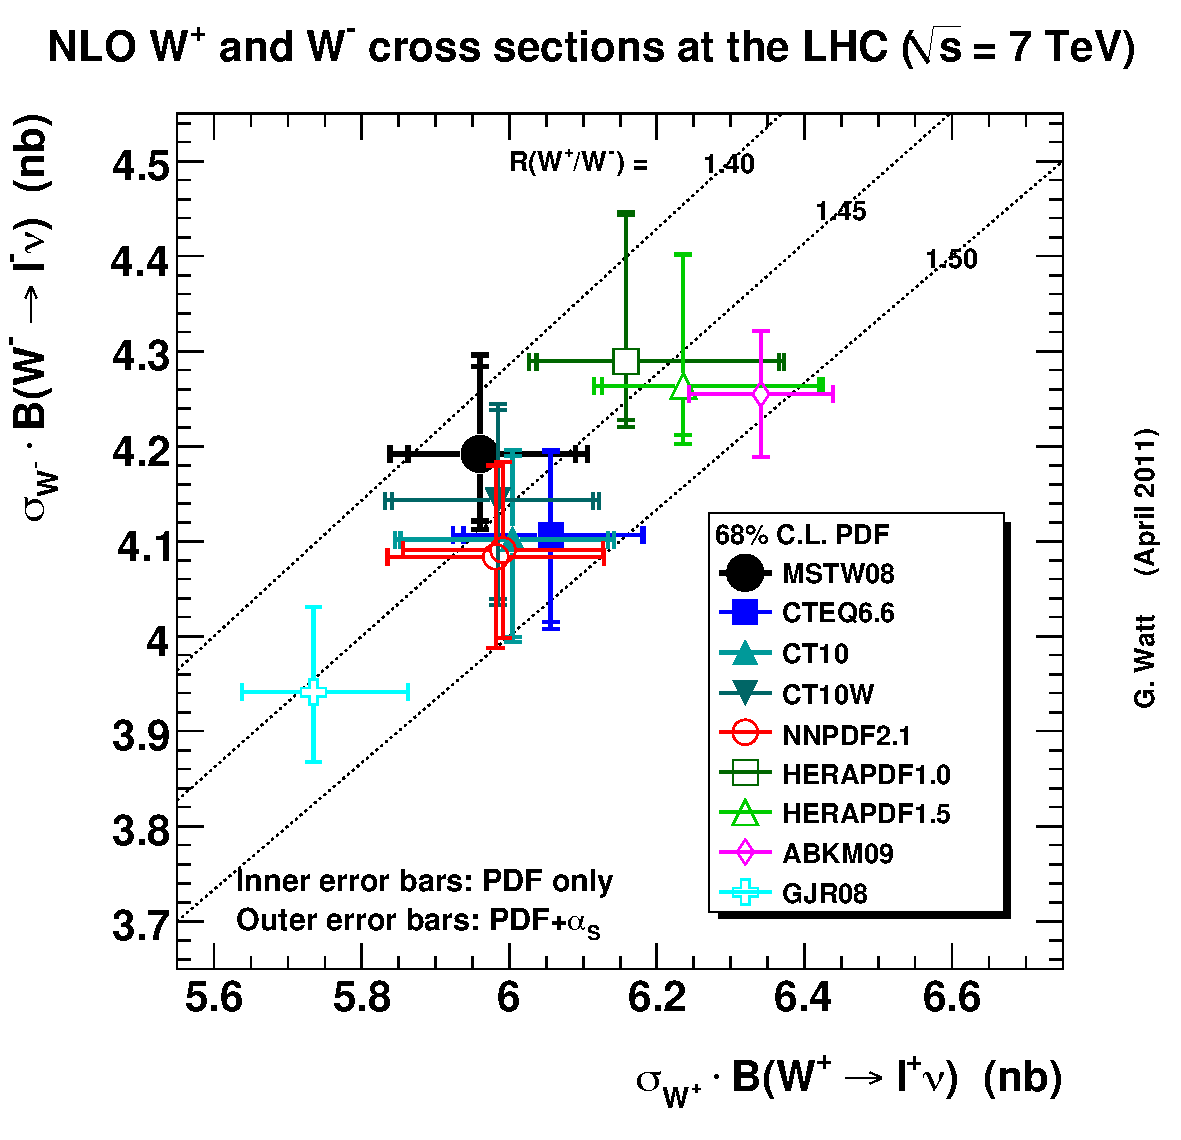
\includegraphics[width=1.0\textwidth]{w+w-lhc7nlo68err.eps}
  \end{column}
  
    \begin{column}{0.55\textwidth}
      \includegraphics[width=1.0\textwidth]{ratiogglumi1_68cl.eps}\\
      \quad { \centering \quad\quad \small \color{blue} G. Watt [hep-ph/1106.5788]}\\

  \end{column}  
  \end{columns}

\end{frame}

\begin{frame}
\frametitle{Parton distribution fitting}

\textbf{Standard approach}
\begin{itemize}
\item<1-> Choose some functional form with a few free parameters for\\ the PDFs at an initial scale, typically
		\be f(x,Q_0^2) = ax^{b}(1-x)^{c}(1+... )\ee
		\vskip10pt

\item<1-> Determine PDF uncertainties by linear error propagation, often with the use of a \textbf{tolerance} criterion.
\end{itemize}
\vskip15pt
\textbf{NNPDF approach}

\begin{itemize}
\item<1->Use of Neural Networks as unbiased and extremely flexible interpolators.
\begin{itemize}
\item<1->Each PDF has 37 free parameters to vary in the fit.
\item<1->Total of 259 free parameters minimises parametrisation bias.
\end{itemize}

\item<1->Monte Carlo approach to uncertainty estimation.
\begin{itemize}
\item<1->Perform an independent NN fit upon an ensemble of artificial data sets.\\
\item<1->Ensemble of PDF replicas faithfully represent the uncertainty in the original experimental data without the need for a tolerance criterion.
\end{itemize}
\end{itemize}

\end{frame}

\begin{frame}
\frametitle{ NNPDF collider only fits }

\underline{Target}: An NNPDF Fit based only upon collider data
\begin{itemize}
\item<1-> Free of contamination from higher twists
\item<1-> No nuclear corrections required
\end{itemize}

 \begin{figure}[b!]
    \begin{center}
      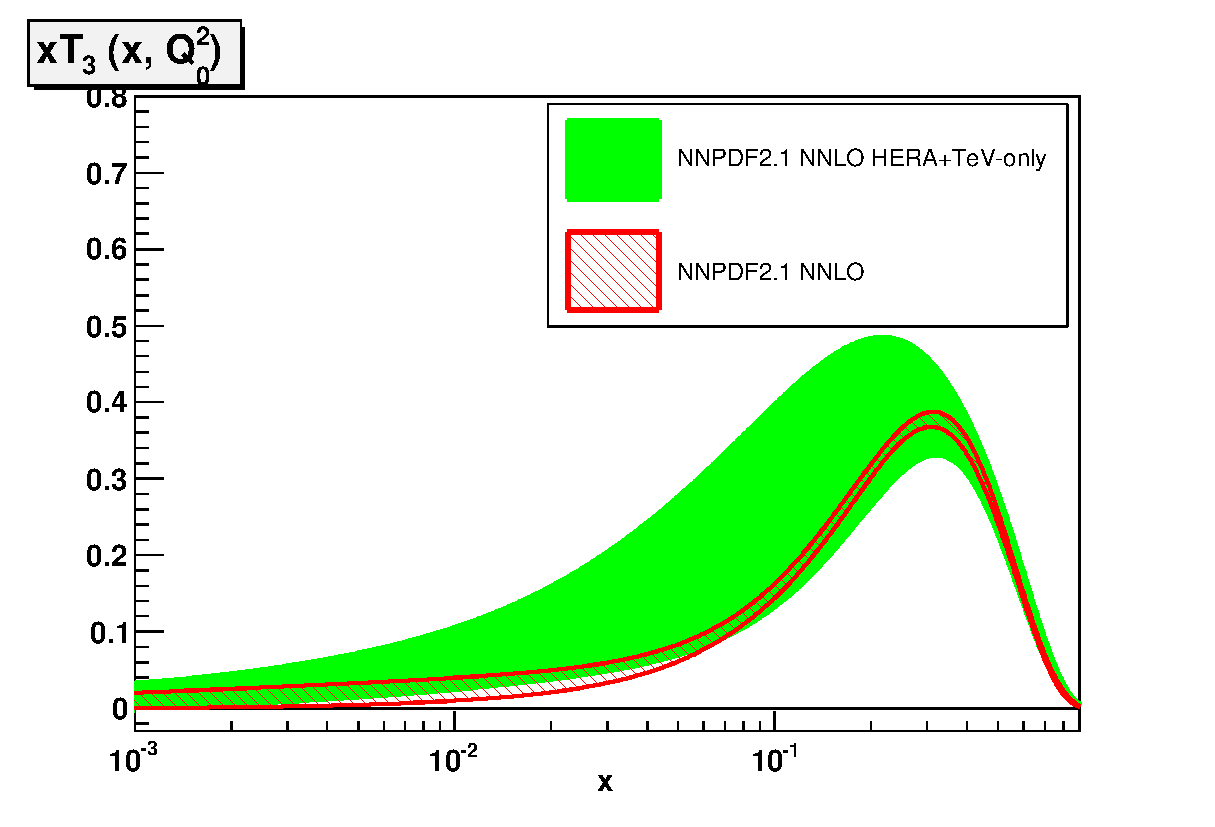
\includegraphics[width=0.50\textwidth]{xT3_Q_2_log-nnpdf21nnlo-collider.eps}
      \includegraphics[width=0.50\textwidth]{xSinglet_Q_2_log-nnpdf21nnlo-collider.eps}
    \end{center}
    \vskip-0.5cm
    \label{fig:pdf-jets}
\end{figure}
\begin{itemize}
\item<1->HERA + Tevatron data provide insufficient constraints in an NNPDF fit
\end{itemize}

\begin{itemize}
\item<1-> LHC data will be crucial to properly constrain future collider only NNPDFs
\end{itemize}
\end{frame}

\begin{frame}
\frametitle{Including new experimental data - reweighting}
How can we add new LHC data to an existing parton set?

\begin{itemize}
		\item<1->Reweight existing Monte Carlo parton set.\\
\end{itemize}
Each replica in the set is assigned a weight based upon it's $\chi^2$ to the new data.
\be \langle\mathcal{O}\rangle_{\mathrm {new}}=\smallfrac{1}{N}\,\sum_{k=1}^{N}w_k\mathcal{O}[f_k], \quad\quad w_k \propto 
(\chi^{2}_k)^{(n-1)/2} 
e^{-\frac{1}{2}\chi^{2}_k}  \ee
\begin{itemize}
		\item<1-> Application: NNPDF2.2 Parton Set   \hfill {\color{blue} [arXiv:1012.0836]}\\
		LHC Electroweak data added by Bayesian Reweighting
\end{itemize}
\vskip10pt

However, reweighting method is impractical for large/constraining data sets.
 Number of effective replicas reduced after reweighting: \be N_{\textrm{ eff}} \equiv \exp \left(\frac{1}{N_{\mathrm{rep}}}\sum_{k=1}^{N_{\mathrm{rep}}}w_k\ln(N_{\mathrm{rep}}/w_k)\right)\ee

\end{frame}


\begin{frame}
\frametitle{Including new experimental data - refitting}
How can we efficiently include LHC data into a full refit?

\underline{Tools}: APPLgrid/FastNLO projects 

\begin{itemize}
\item<1-> Precompute and store MC Weights on an interpolation grid
\end{itemize}
\begin{equation}
\label{eq:applconv}
\sigma = \sum_p \sum_{l=0}^{N_{\mathrm{sub}}} \sum_{\alpha,\beta}^{N_x} \sum_{\tau}^{N_{Q}}
W_{\alpha\beta\tau}^{(p)(l)} \, \left( \frac{\alpha_s\left(Q^2_{\tau}\right)}{2\pi}\right)^{p}
F^{(l)}\left(x_{\alpha}, x_{\beta},  Q^2_{\tau}\right)
\end{equation}
PDF Evolution in the FastKernel method is a similar procedure,
\be f_i(x_{\alpha},Q^2_\tau) =  \sum_\beta^{N_{x}} \sum_{j}^{N_{\mathrm{pdf}}} A^{\tau}_{\alpha\beta ij}N^0_j(x_{\beta} )\ee 
\underline{Idea}: Combine weight grids with evolution grids 

  \be \sigma= \sum_{\alpha,\beta}^{N_x}\sum_{i,j}^{N_{\mathrm{pdf}}} \sigma_{\alpha\beta i j}N_i^0(x_\alpha)N_j^0(x_\beta)\ee
 \begin{itemize}
\item<1-> Precomputing all $Q^2$ dependence leads to extremely efficient calculations.
\end{itemize}\end{frame}

\begin{frame}
\frametitle{NNPDF2.3 - LHC Data}
\begin{itemize}
\item<1->{ \small The NNPDF2.3 dataset contains all LHC data with published correlation matrices }
 \begin{itemize}
 \item<1->  $36$ pb$^{-1}$ ATLAS Inclusive jet measurements \hfill  {\color{blue}[arxiv:1112.5141]}
  \item<1->  $35$ pb$^{-1}$  ATLAS W lepton and Z differential distributions \hfill{\color{blue}[arxiv:1109.5141]}
   \item<1->  $37$ pb$^{-1}$ LHCb W lepton and Z differential distributions \hfill {\color{blue}[arxiv:1204.1620]}
  \item<1-> $840$ pb$^{-1}$ CMS  W electron asymmetry \hfill {\color{blue}[arxiv:1206.2598]}

\end{itemize}
\end{itemize}

\begin{columns}
  \begin{column}{0.5\textwidth}
   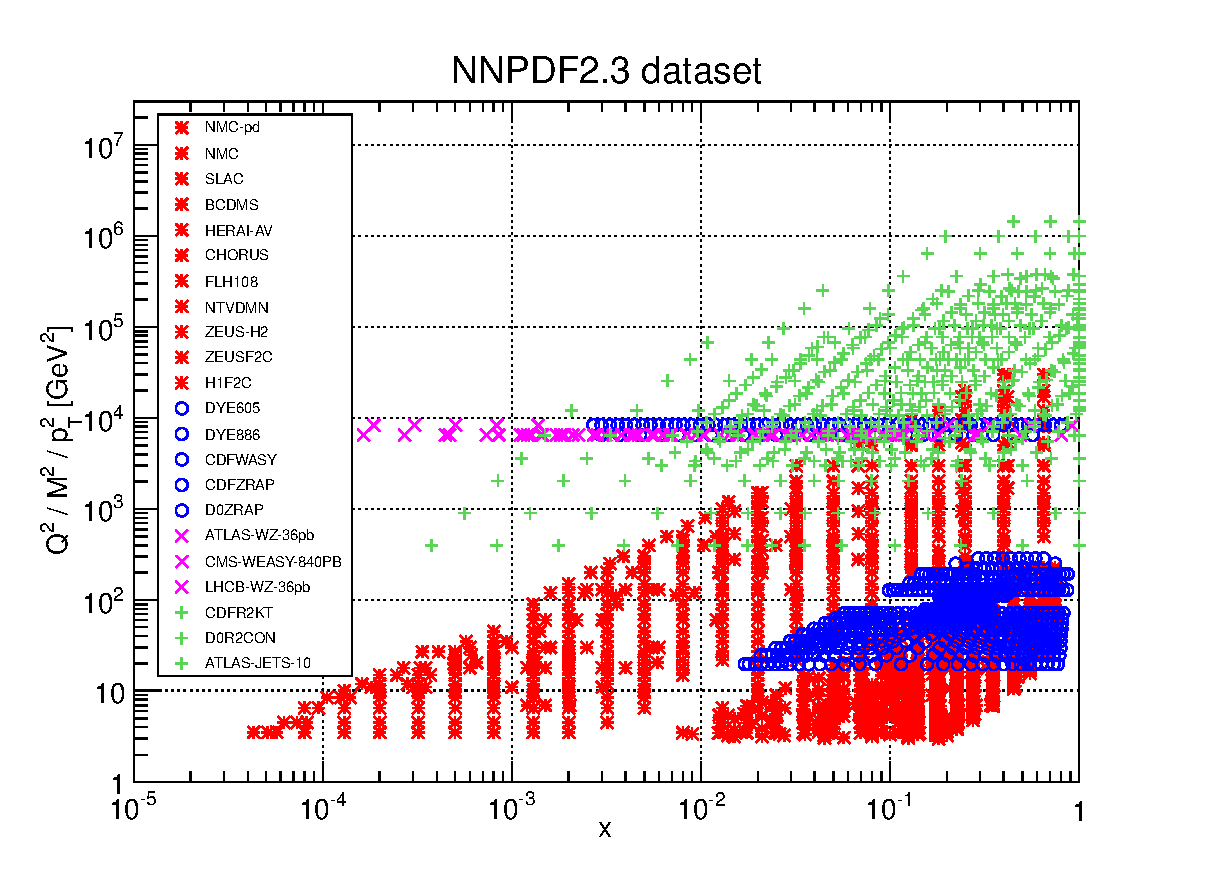
\includegraphics[width=1.0\textwidth]{kin23}
  \end{column}

  \begin{column}{0.5\textwidth}
    \small
\underline{Methodological Improvements}\\
\vskip10pt
Improved dynamical stopping.\\
Expanded genetic algorithm minimisation.\\
Improved training/validation partitioning.

\begin{table}
\scriptsize
\begin{tabular}{|c|c|c||c|c|}
\hline 
& \multicolumn{2}{c||}{\bf NNPDF2.1} & \multicolumn{2}{|c|}{\bf NNPDF2.3}  \\
\hline 
\hline 
  & NLO & NNLO  & NLO  & NNLO  \\
\hline 
Fit Quality  & 1.16 & 1.16  & 1.14 & 1.15     \\
\hline
\end{tabular}
\end{table}

  \end{column}
\end{columns}









\begin{itemize}
\item<2->Also in the NNPDF2.3 family
\begin{itemize}
 \item<1-> NNPDF2.3 noLHC:  same dataset as NNPDF2.1, with improved methodology.
  \item<1->  NNPDF2.3 Collider only: dataset restricted to HERA, Tevatron and LHC data.
\end{itemize}
\end{itemize}
\end{frame}

\begin{frame}
\frametitle{Impact of LHC EW vector boson data}
 \begin{figure}[b!]
    \begin{center}
      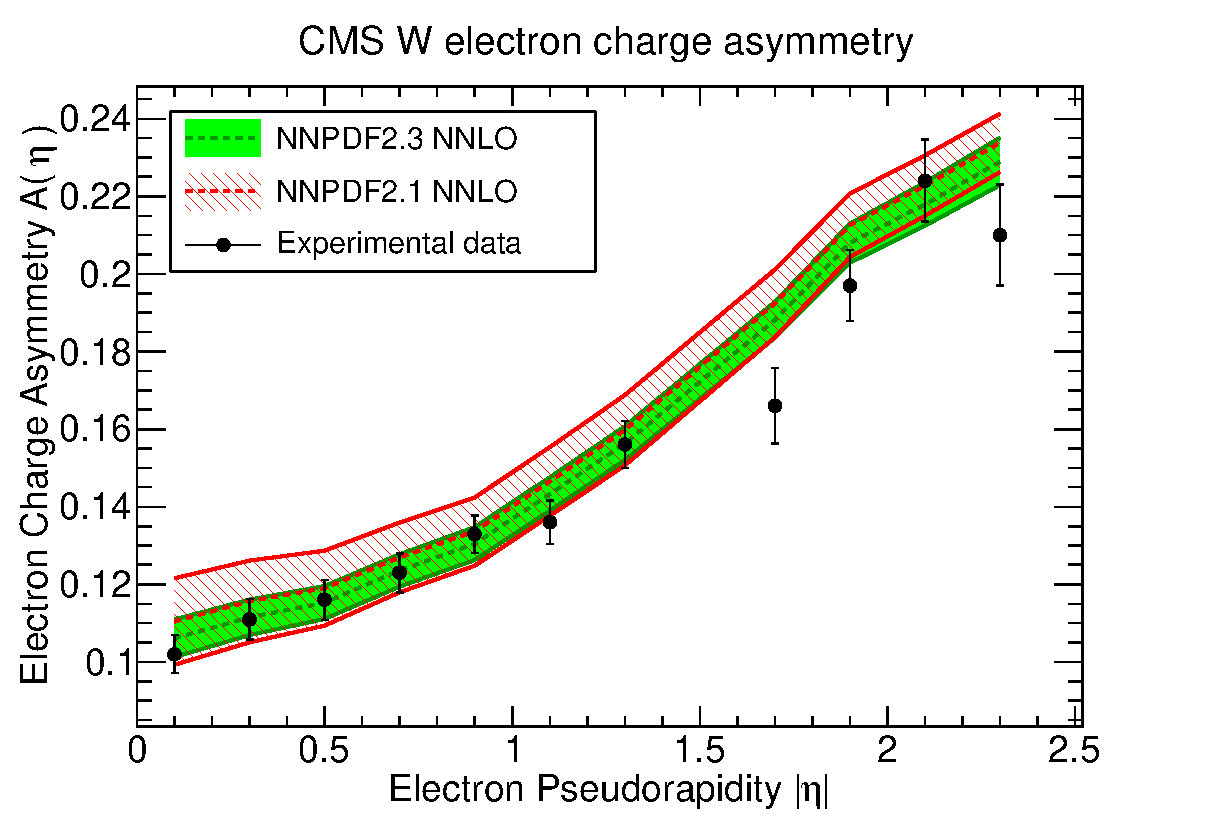
\includegraphics[width=0.50\textwidth]{CMSWEASY840PB_0.eps}
      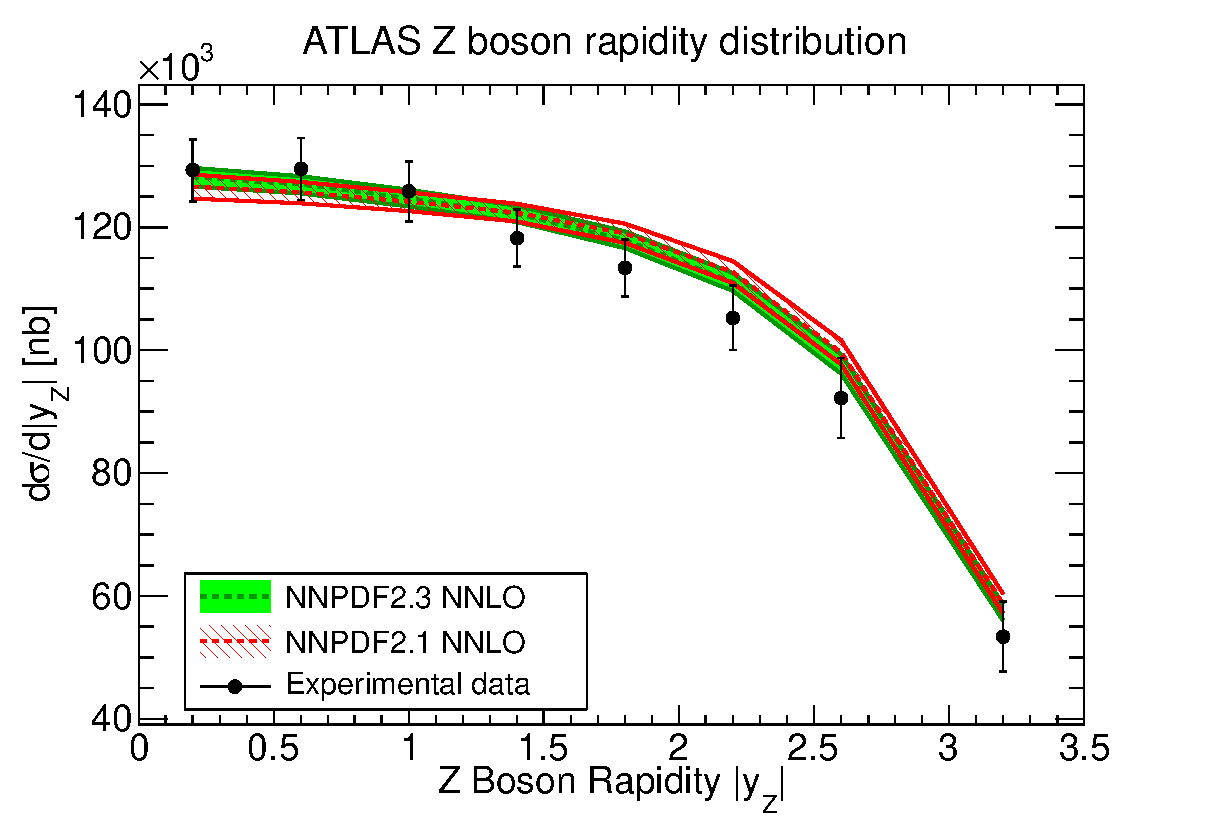
\includegraphics[width=0.50\textwidth]{ATLASWZRAP36PB_2.eps}
    \end{center}
    \vskip-0.5cm
    \label{fig:pdf-jets}
\end{figure}

\begin{table}
\small
\begin{tabular}{|c||c|c||c|c|}
\hline 
& \multicolumn{2}{c||}{\bf NNPDF2.1} & \multicolumn{2}{|c|}{\bf NNPDF2.3}  \\
\hline 
\hline 
Experiment  & NLO & NNLO  & NLO  & NNLO  \\
\hline
ATLAS W/Z Distributions & {\it 1.63} & {\it 2.15}  & 1.29  &  1.39   \\
CMS $W_e$ Asymmetry  & {\it 2.26} & {\it 1.45}  & 1.04 & 0.98   \\
LHCb W/Z Distributions & {\it 1.16} &  {\it 1.23} & 1.14  & 1.14   \\
\hline
\end{tabular}
\end{table}


\end{frame}

\begin{frame}
\frametitle{Impact of ATLAS inclusive jet data}
 \begin{figure}[b!]
    \begin{center}
      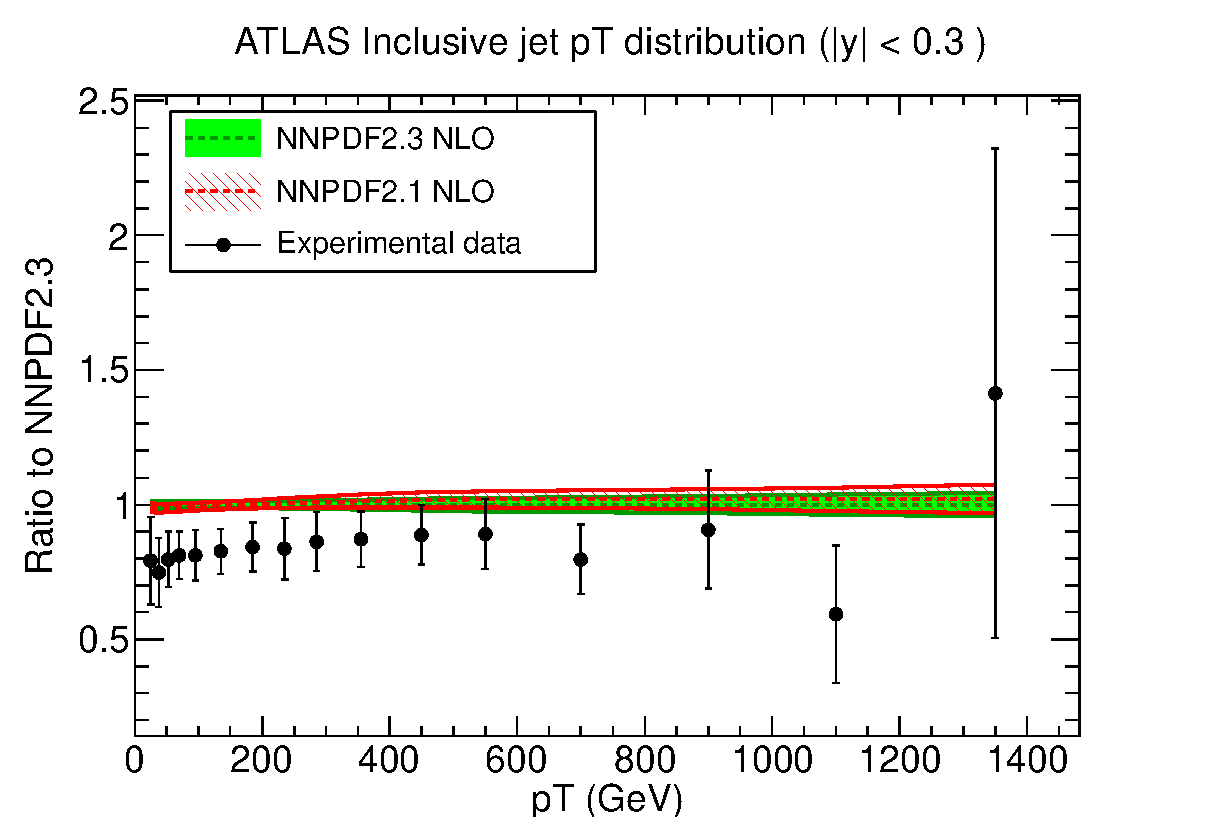
\includegraphics[width=0.50\textwidth]{ATLASR04JETS36PB_0}
      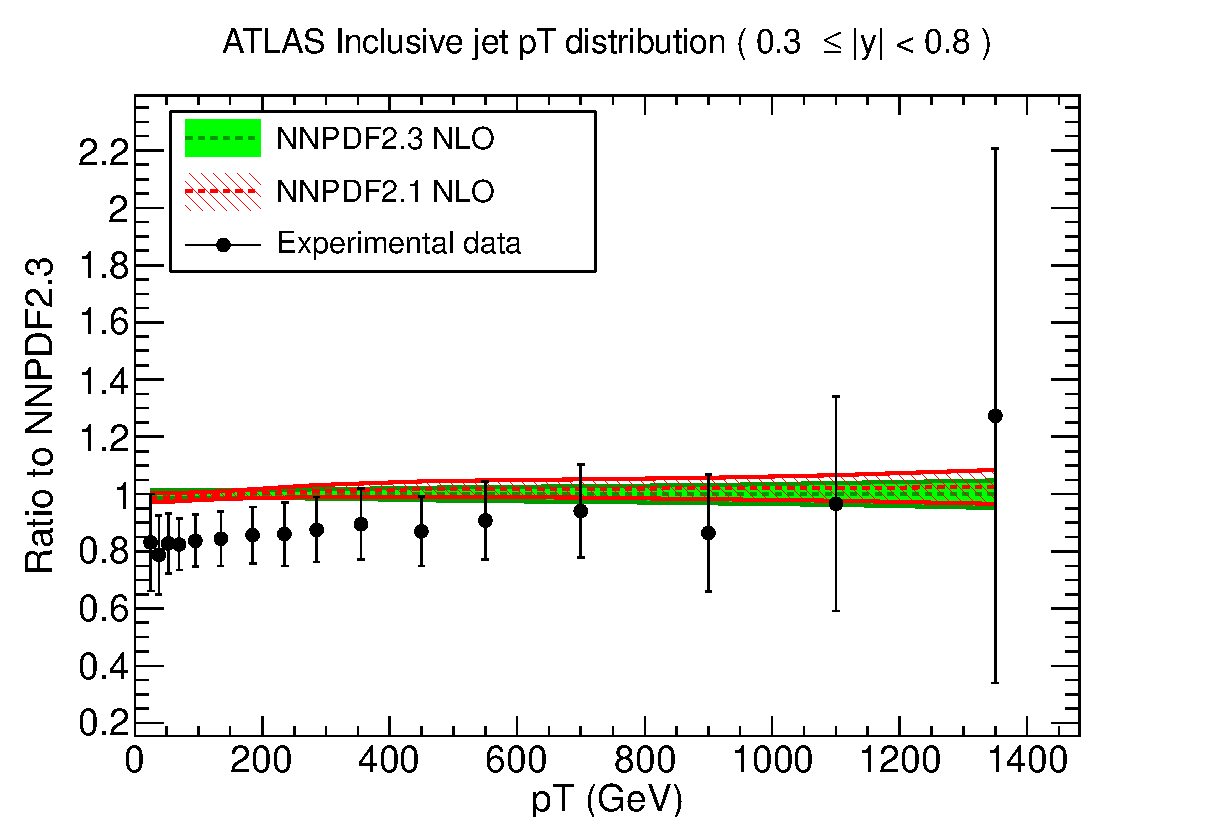
\includegraphics[width=0.50\textwidth]{ATLASR04JETS36PB_1}
    \end{center}
    \vskip-0.5cm
    \label{fig:pdf-jets}
\end{figure}
\begin{table}
\small
\begin{tabular}{|c||c|c||c|c|}
\hline 
& \multicolumn{2}{c||}{\bf NNPDF2.1} & \multicolumn{2}{|c|}{\bf NNPDF2.3}  \\
\hline 
\hline 
Experiment  & NLO & NNLO  & NLO  & NNLO  \\ 
\hline
ATLAS Inclusive Jets  & {\it 1.41} & {\it 1.28}  & 1.29  &  1.21   \\
\hline
\end{tabular}
\end{table}


\end{frame}

\begin{frame}
\frametitle{NNPDF2.3 vs NNPDF2.1}
 \begin{figure}[b!]
    \begin{center}
      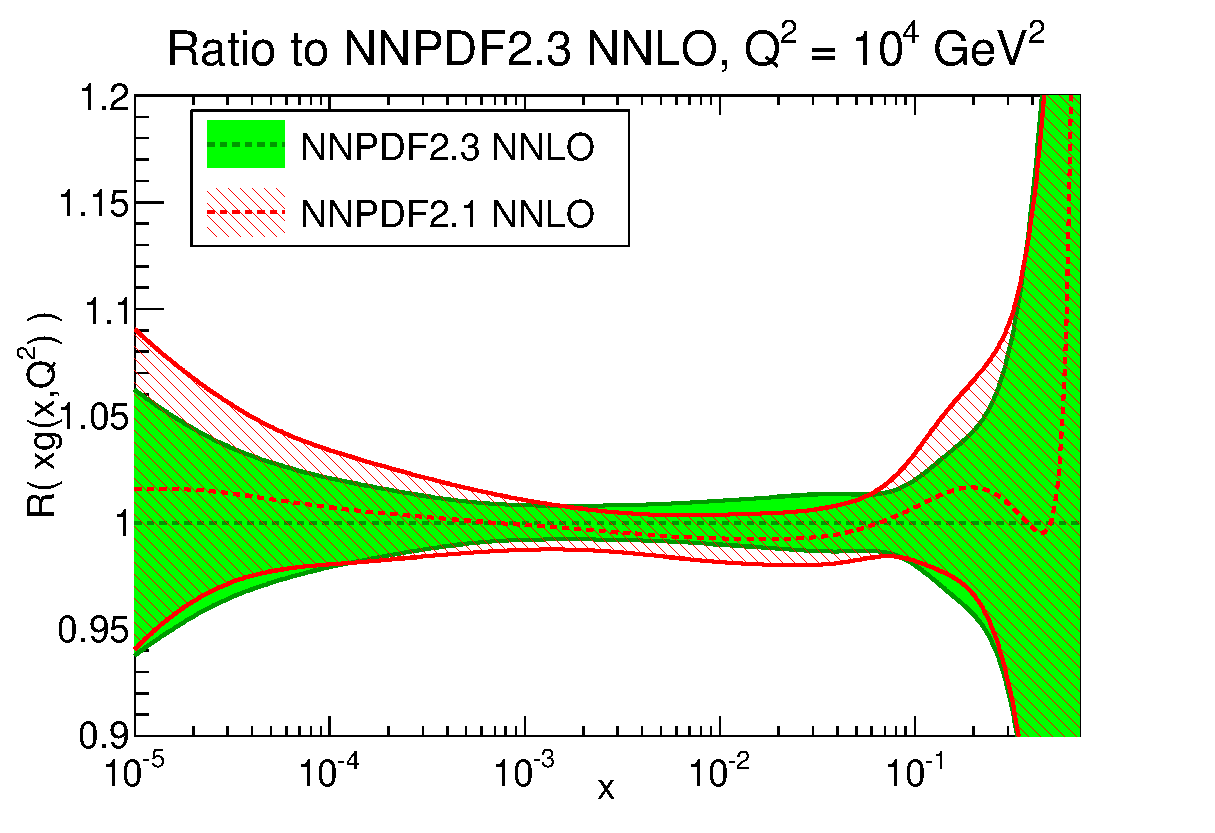
\includegraphics[width=0.50\textwidth]{xg_Q_10000_log-rat-21-vs-23-nnlo}
      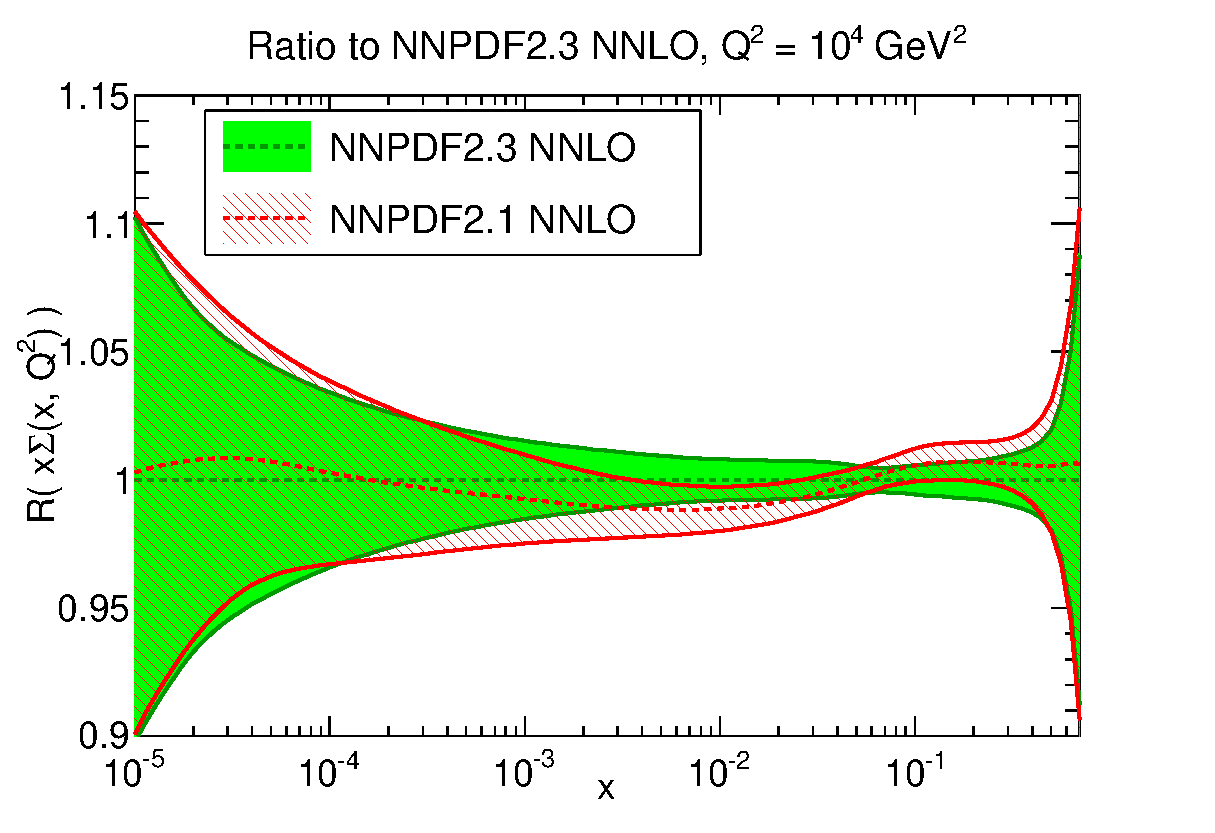
\includegraphics[width=0.50\textwidth]{xSinglet_Q_10000_log-rat-21-vs-23-nnlo}
    \end{center}
    \vskip-0.5cm
    \label{fig:pdf-jets}
\end{figure}

 \begin{figure}[b!]
    \begin{center}
      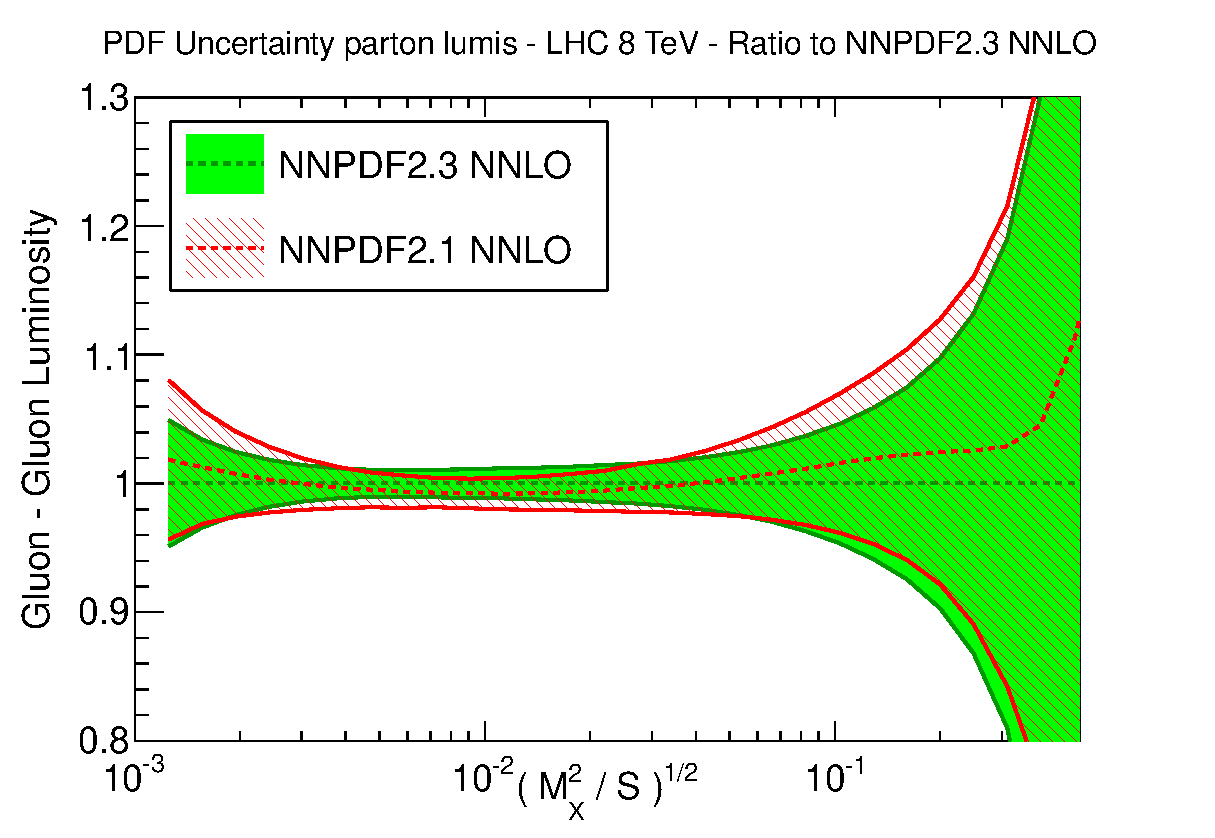
\includegraphics[width=0.50\textwidth]{gg_S_6_4e+07-rat-8tev}
      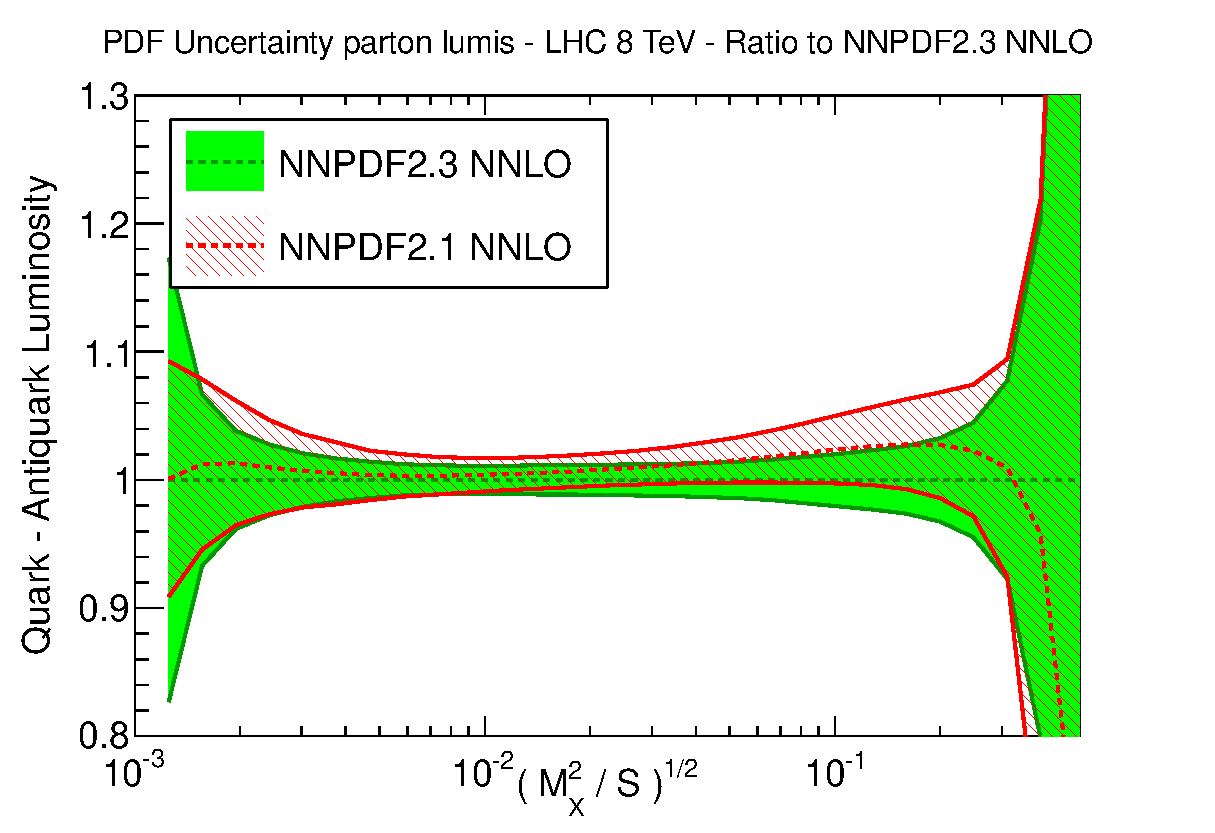
\includegraphics[width=0.50\textwidth]{qq_S_6_4e+07-rat-8tev}
    \end{center}
    \vskip-0.5cm
    \label{fig:pdf-jets}
\end{figure}

\vskip15pt
\center{Modest reduction in uncertainties on parton luminosities.}

\end{frame}


\begin{frame}
\frametitle{Collider only PDFs with LHC data}
 \begin{figure}[b!]
    \begin{center}
      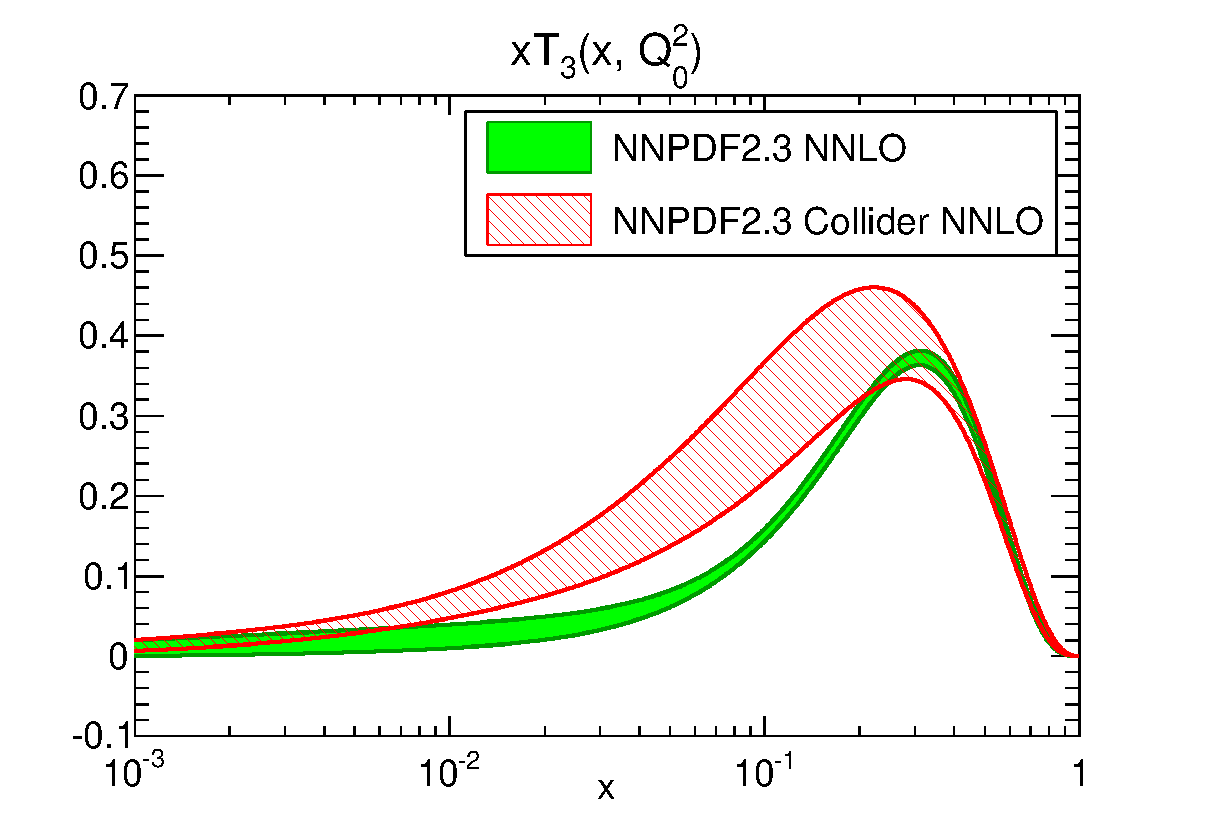
\includegraphics[width=0.50\textwidth]{xT3_Q_2_log-23-vs-23coll-nnlo.eps}
      \includegraphics[width=0.50\textwidth]{xSinglet_Q_2_log-23-vs-23coll-nnlo}
    \end{center}
    \vskip-0.5cm
    \label{fig:pdf-jets}
\end{figure}
\vskip10pt
\begin{itemize}
\item<1-> LHC data providing some constraint upon existing collider only NNPDF determination.
\item<1-> Collider only uncertainties remain large for flavour separation, strangeness.

\end{itemize}

\end{frame}


 
\begin{frame}
\frametitle{Summary}

\center {\textbf{LHC data in NNPDF2.3 }}\vskip10pt
\begin{itemize}\small
\item<1-> The NNPDF2.3 parton set is the new standard PDF set of the NNPDF collaboration. \vskip10pt
\item<1-> NNPDF2.3 provides a determination of parton distributions with a faithful representation of the experimental uncertainties, and without parametrisation bias.  \vskip10pt

\item<1-> The FastKernel method is utilised to perform fully NLO QCD calculations, enabling
the efficient inclusion of LHC electroweak boson production and inclusive jet datasets into an NNPDF fit.  \vskip10pt

\item<1-> LHC data provides a valuable constraint upon PDFs,  reducing the uncertainty in the gluon, and modifying the shape of the light quark pdfs.

\end{itemize}

\end{frame}

\begin{frame}
    \begin{center}
      BACKUPS
    \end{center}
\end{frame}

\begin{frame}
\frametitle{Determination of $R_s$}

\be
\label{eq:rs}
r_s (x,Q^2)=\frac{ s(x,Q^2)+\bar{s}(x,Q^2) }{ 2 \bar{d}(x,Q^2) } 
\ee \vskip15pt
 \begin{figure}[b!]
    \begin{center}
      \includegraphics[width=0.50\textwidth]{rs-10000.eps}
      \includegraphics[width=0.50\textwidth]{rs-2.eps}
    \end{center}
    \vskip-0.5cm
    \label{fig:pdf-jets}
\end{figure}

\end{frame}

%
%
%
%\begin{frame}
%\small
%\frametitle{Special features of NNPDF approach}
%\textbf{Minimisation by genetic algorithms}\\
%\underline{Problem}: Very large parameter space, $\chi2$ highly nonlocal. \begin{itemize}
%\item<1-> Minimisation is challenging.
%\end{itemize}\underline{Solution}: Genetic Algorithms (GA)
%\begin{itemize}
%\item<1-> Generate mutations of fit parameters.
%\item<1-> Select those mutations that minimise figure of merit.
%\end{itemize}
%\vskip10pt
%\textbf{ Dynamical fit stopping by cross-validation}\\
%\underline{Problem}:  extremely flexible parameterisations are prone to \emph{overfitting}.
%\\
%\begin{itemize}
%\item<1->Fit has so many parameters, the minimum $\chi^2$ corresponds to a fit not only to
%the data, but also statistical noise.
%\end{itemize}
%\underline{Solution}:  dynamical stopping by \emph{Cross Validation}.
%\begin{itemize}
%\item<1-> Split the dataset into a training set and a validation set.
%\item<1-> Use the training set for minimisation, monitor the $\chi^2$ to the validation set.
%\item<1-> Stop the fit when the $\chi^2$ to the validation set starts to increase while
%the $\chi^2$ to training set is still decreasing.
%
%\end{itemize}
%
%
%
%\end{frame}
%
%\begin{frame}
%\frametitle{Cross Validation}
% \begin{figure}[b!]
%    \begin{center}
%      \includegraphics[width=0.9\textwidth]{chi2ite-1004-NMC-pd.eps}
%    \end{center}
%\end{figure}
%\end{frame}
%
%\begin{frame}
%\frametitle{Unweighting procedure}
%\begin{columns}
%  \begin{column}{0.5\textwidth}
%\begin{figure}
%  \epsfig{width=0.7\textwidth,figure=unwplot-1.eps,angle=-90}\\
%\end{figure}
%  \end{column}
%  \begin{column}{0.5\textwidth}
%\begin{figure}
%  \epsfig{width=0.7\textwidth,figure=unwplot-2.eps,angle=-90}
%\end{figure}
%  \end{column}
%\end{columns}
%\end{frame}
%

% End of slides
\end{document} 